\documentclass{beamer}
\usepackage{amsfonts,amsmath,oldgerm}
\usetheme{sintef}
\usepackage{xeCJK}
\usepackage{graphicx}

% 自定义页码显示
\setbeamertemplate{footline}[frame number]

\newcommand{\testcolor}[1]{\colorbox{#1}{\textcolor{#1}{test}}~\texttt{#1}}

\usefonttheme[onlymath]{serif}

\titlebackground*{assets/background}

\newcommand{\hrefcol}[2]{\textcolor{cyan}{\href{#1}{#2}}}

\title{Benchmarking ensemble machine learning algorithms for multi-class, multi-omics data integration in clinical outcome prediction}
\subtitle{A Comparative Study of Late Integration Methods}
\author{尹超}
\date{2025.08.19}

\begin{document}
\maketitle
\addtocounter{framenumber}{-1}

\section{Introduction}

\begin{frame}{Research Overview}
\begin{itemize}
\item \alert{Problem}: Multi-omics data integration for clinical outcome prediction
\item \alert{Challenge}: High dimensionality, heterogeneous data, small sample sizes
\item \alert{Solution}: Ensemble machine learning with late integration strategies
\item \alert{Application}: Hepatocellular carcinoma, breast cancer, IBD
\end{itemize}
\end{frame}

\begin{frame}{Motivation}
\begin{columns}
\begin{column}{0.6\textwidth}
\begin{itemize}
\item Multi-omics data provides \alert{complementary information}
\item Better understanding of disease mechanisms
\item Improved clinical outcome prediction
\item Challenges in multi-omics integration:
  \begin{itemize}
  \item Curse of dimensionality
  \item Heterogeneous data types
  \item Missing values and batch effects
  \end{itemize}
\end{itemize}
\end{column}
\begin{column}{0.4\textwidth}
\begin{block}{Benefits}
\begin{itemize}
\item Enhanced accuracy
\item Novel biomarker discovery
\item Disease subtyping
\item Therapeutic targets
\end{itemize}
\end{block}
\end{column}
\end{columns}
\end{frame}

\section{Background}

\begin{frame}{Data Integration Strategies}
\begin{itemize}
\item \alert{Early Integration} (Feature-level fusion)
  \begin{itemize}
  \item Concatenate all omics data
  \item Train single classifier
  \item Problem: Exacerbates high dimensionality
  \end{itemize}
\item \alert{Intermediate Integration}
  \begin{itemize}
  \item Transform to common representation
  \item Difficult clinical interpretation
  \end{itemize}
\item \alert{Late Integration} (Decision-level fusion)
  \begin{itemize}
  \item Train separate models on each modality
  \item Aggregate results for final prediction
  \item \textbf{Focus of this work}
  \end{itemize}
\end{itemize}
\end{frame}

\begin{frame}{Advantages of Late Integration}
\begin{itemize}[<+->]
\item \alert{Reduces dimensionality} - separate models per modality
\item \alert{Flexible} - different ML models for each modality
\item \alert{Addresses heterogeneity} - tailored preprocessing
\item \alert{Reduces overfitting} - smaller feature spaces
\item \alert{Lower computational complexity}
\item \alert{Modality-specific optimization}
\end{itemize}
\end{frame}

\section{Methods}

\begin{frame}{Ensemble Methods Overview}
  \begin{figure}[H]
    \centering
    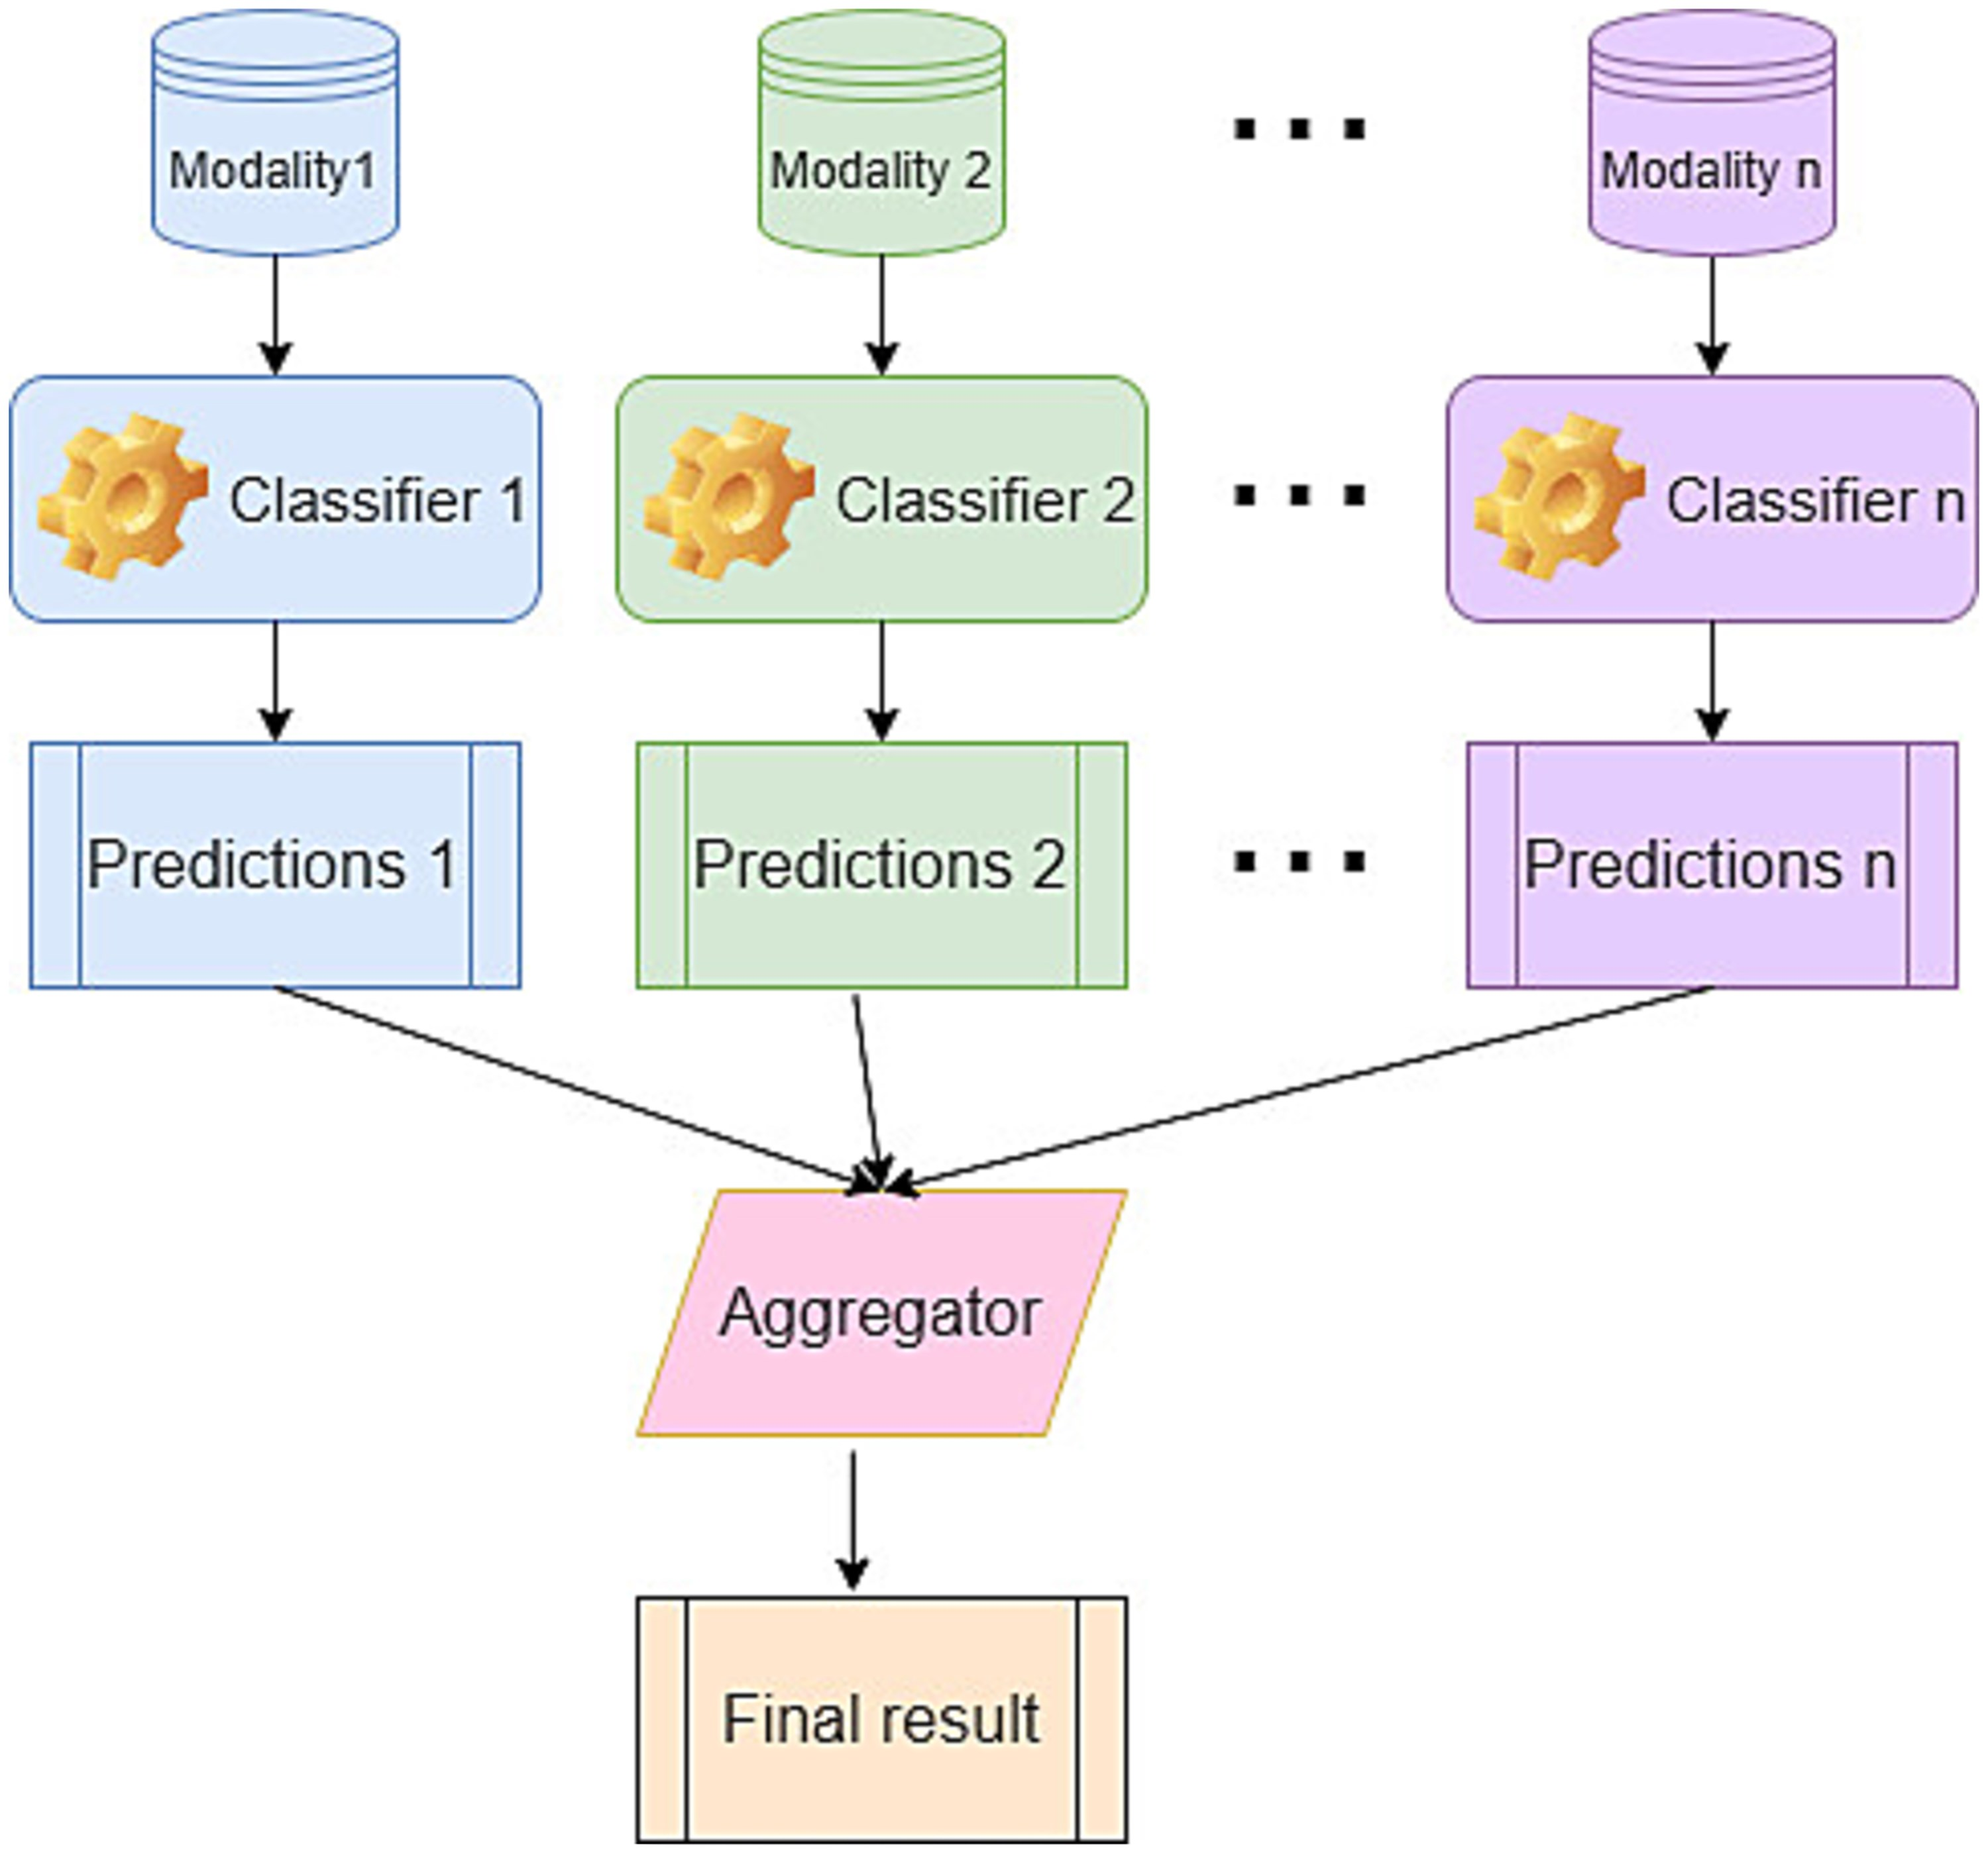
\includegraphics[width=0.52\textwidth]{assets/classifier.png}
  \end{figure}
\end{frame}

\begin{frame}{Ensemble Methods Evaluated}
\begin{enumerate}
\item \alert{Voting Ensemble}
  \begin{itemize}
  \item Hard vote (majority)
  \item Soft vote (probability averaging)
  \end{itemize}
\item \alert{Meta Learner}
  \begin{itemize}
  \item Random forest as meta-classifier
  \end{itemize}
\item \alert{Multi-modal AdaBoost}
  \begin{itemize}
  \item Hard vote, soft vote, meta learner variants
  \end{itemize}
\item \alert{PB-MVBoost}
  \begin{itemize}
  \item Balances accuracy and diversity
  \end{itemize}
\item \alert{Mixture of Experts}
  \begin{itemize}
  \item Novel application with gating function
  \end{itemize}
\end{enumerate}
\end{frame}


\begin{frame}{Data Processing Pipeline}
\framesubtitle{Comprehensive preprocessing approach}

\begin{figure}[H]
  \centering
  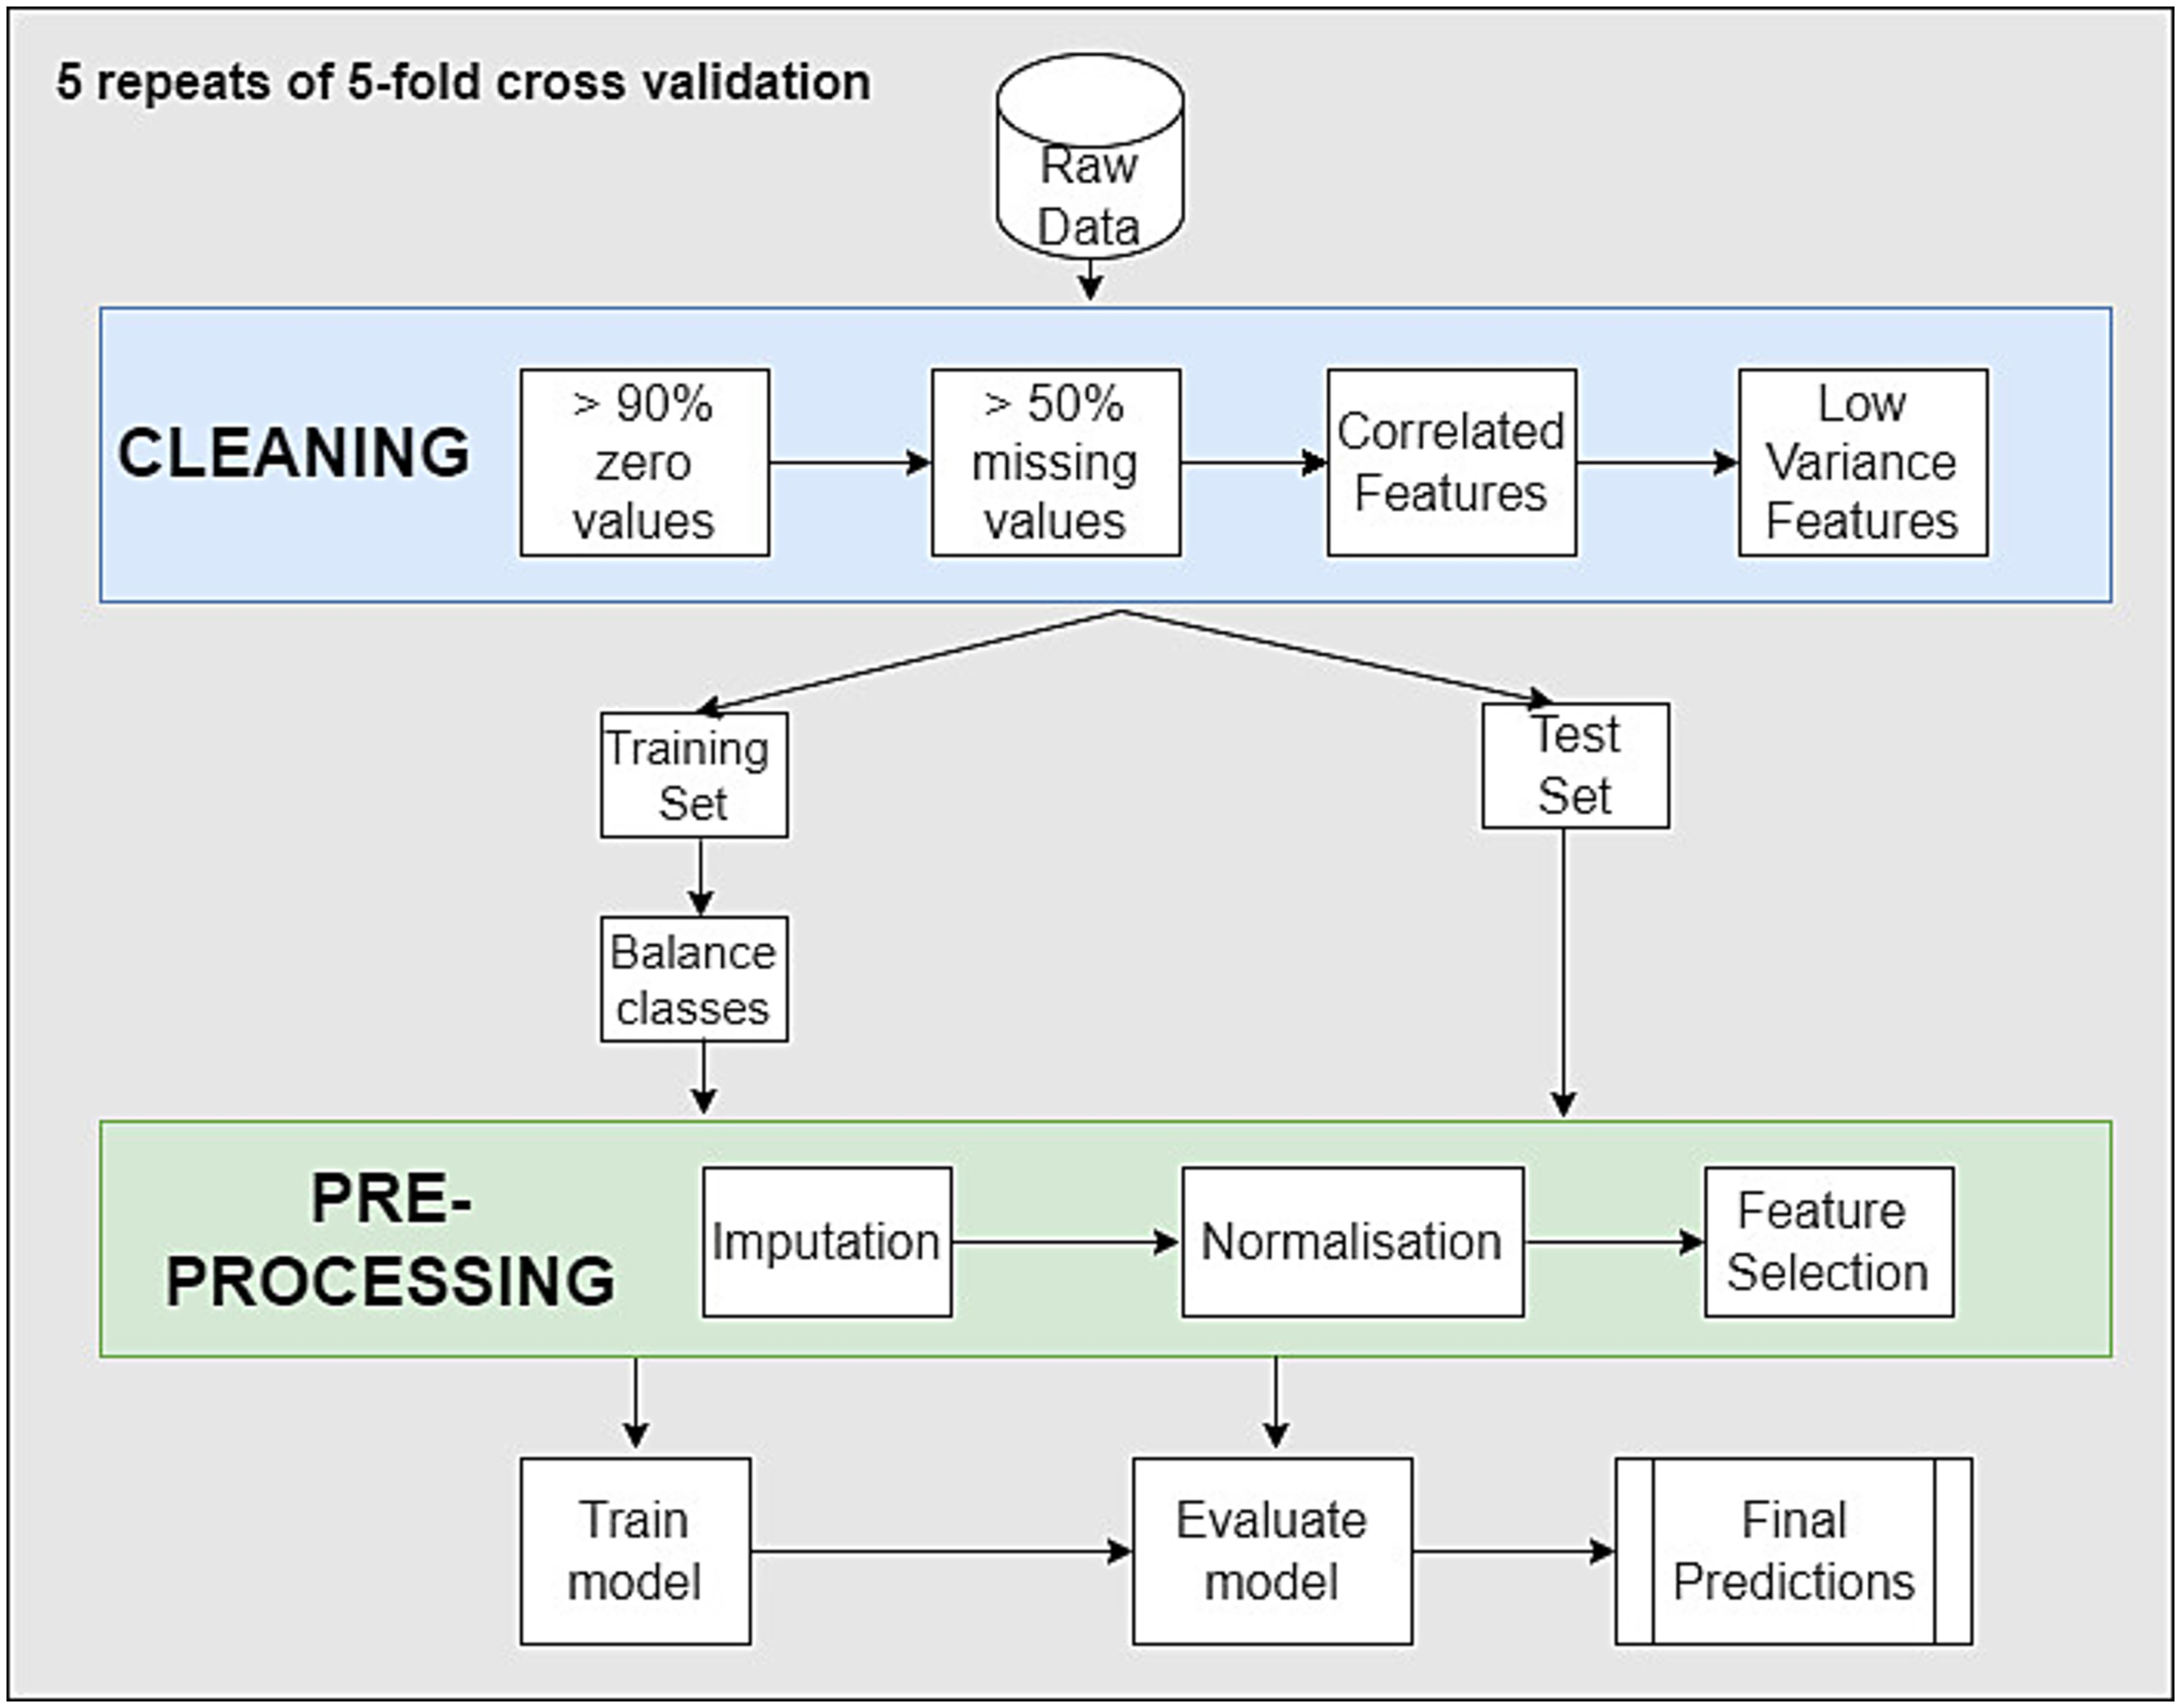
\includegraphics[width=0.6\textwidth]{assets/data_processing_pipeline.png}
  \caption{Overview of the data processing pipeline}
\end{figure}

\end{frame}


\begin{frame}{Data Processing Pipeline}
\framesubtitle{Comprehensive preprocessing approach}
\begin{block}{Filtering Steps}
\begin{itemize}
\item Remove features with >50\% missing values
\item Remove features with >90\% zero values
\item Eliminate correlated features
\item Retain top 500 highest variance features if needed
\end{itemize}
\end{block}

\begin{block}{Preprocessing Steps}
\begin{itemize}
\item \alert{Balancing}: SMOTE for imbalanced datasets
\item \alert{Imputation}: MICE or k-NN for missing values
\item \alert{Normalization}: CPM + log transformation for RNA/DNA
\item \alert{Feature Selection}: Boruta algorithm with GBM
\end{itemize}
\end{block}
\end{frame}

\begin{frame}{Datasets}
\begin{figure}[H]
  \centering
  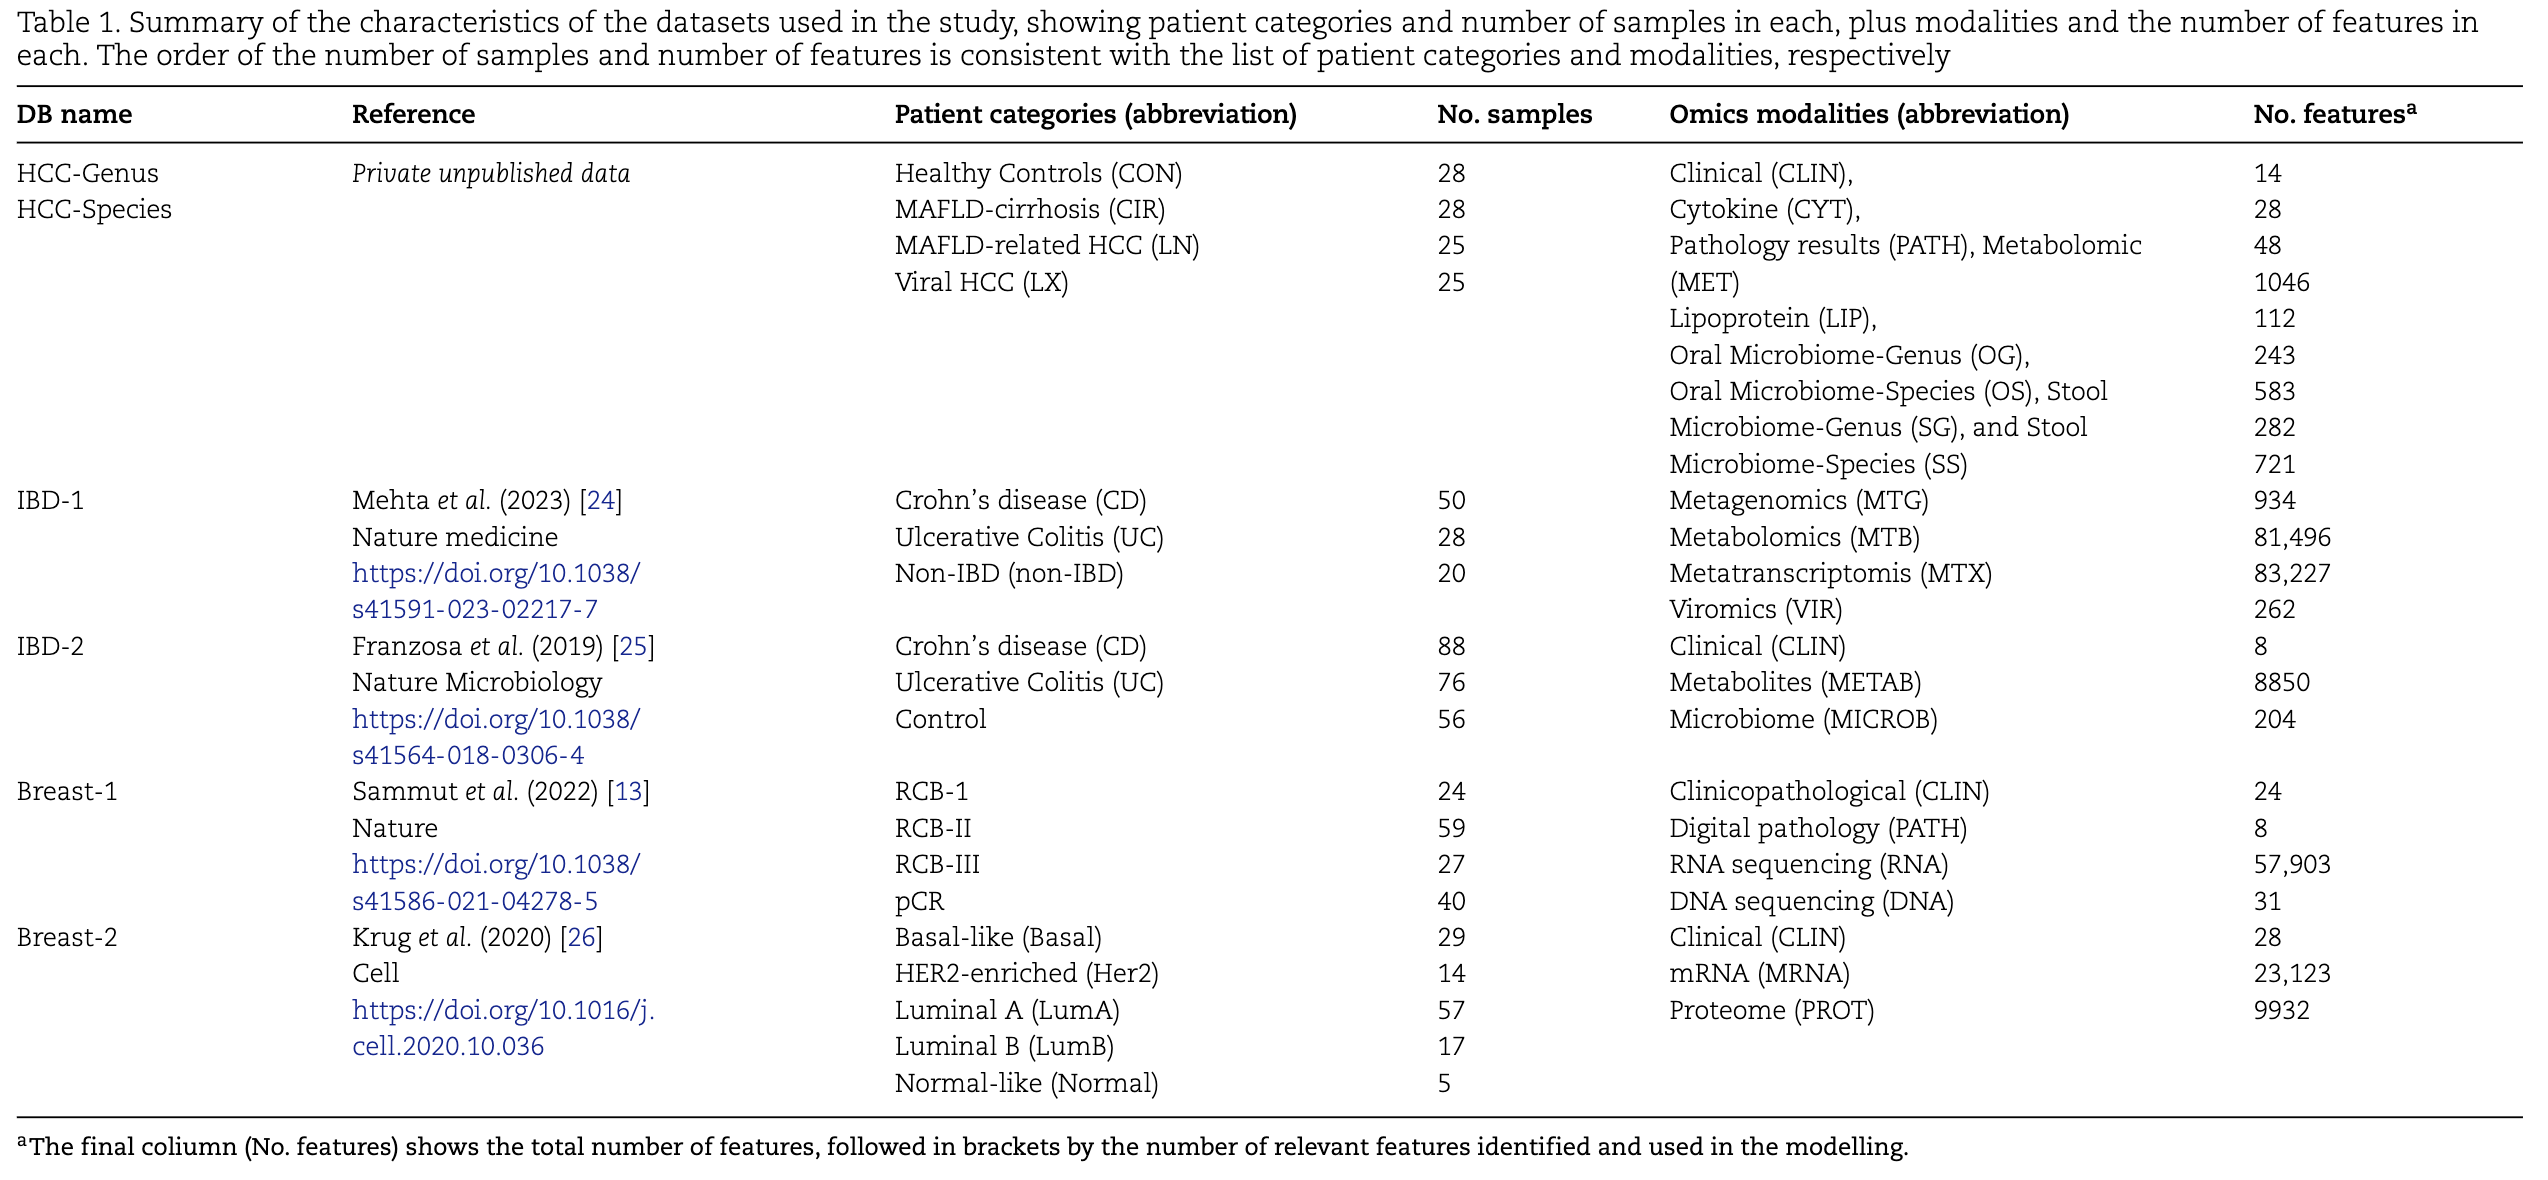
\includegraphics[width=1\textwidth]{assets/datasets.png}
\end{figure}
\end{frame}

\begin{frame}
  \frametitle{Voting Ensemble}
  \begin{figure}[H]
    \centering
    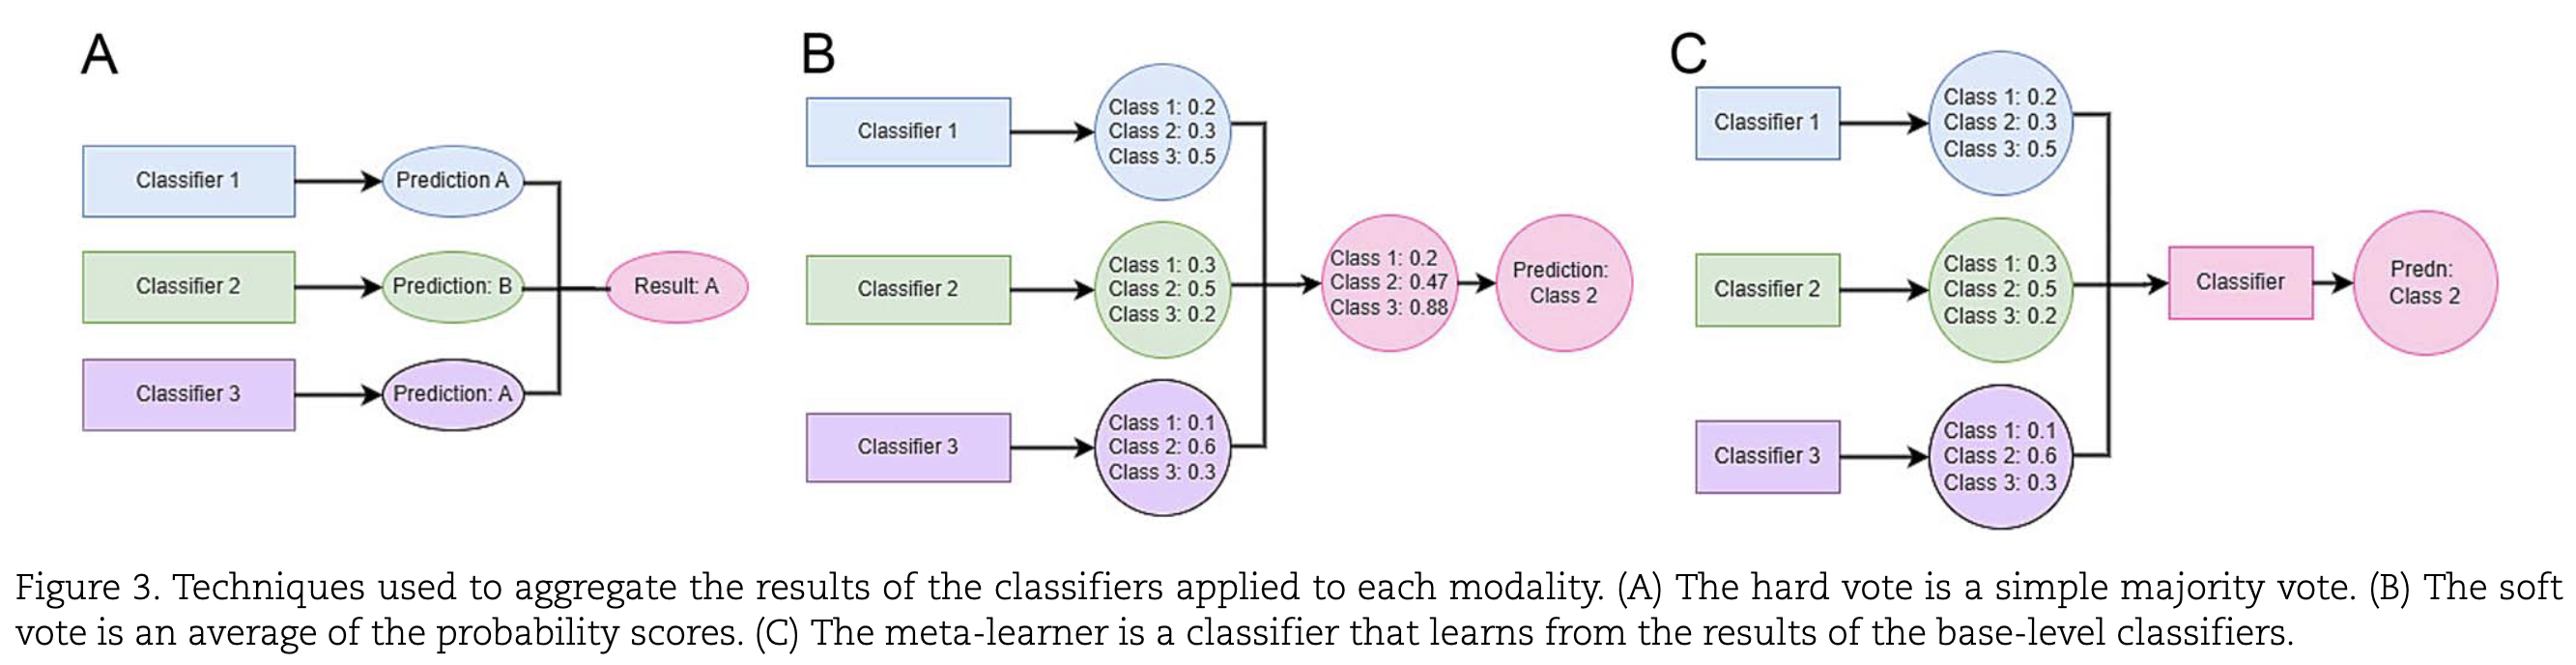
\includegraphics[width=1\textwidth]{assets/vote_meta.png}
  \end{figure}
\end{frame}

\section{Results}

\begin{frame}{Performance Results}
\begin{itemize}
\item \alert{Best performers}: PB-MVBoost and AdaBoost with soft vote
\item \alert{Peak performance}: AUC up to 0.85 (HCC dataset)
\item Multi-modal methods \alert{outperformed} individual modalities in most cases
\item \alert{Soft vote consistently better} than hard vote
\end{itemize}

\begin{block}{Key Finding}
Boosting methods excel due to:
\begin{itemize}
\item Reduced overfitting
\item Modality weighting
\item Suited for high-dimensional, small-sample data
\end{itemize}
\end{block}
\end{frame}

\begin{frame}{Evaluation Metrics}
\begin{figure}[H]
  \centering
  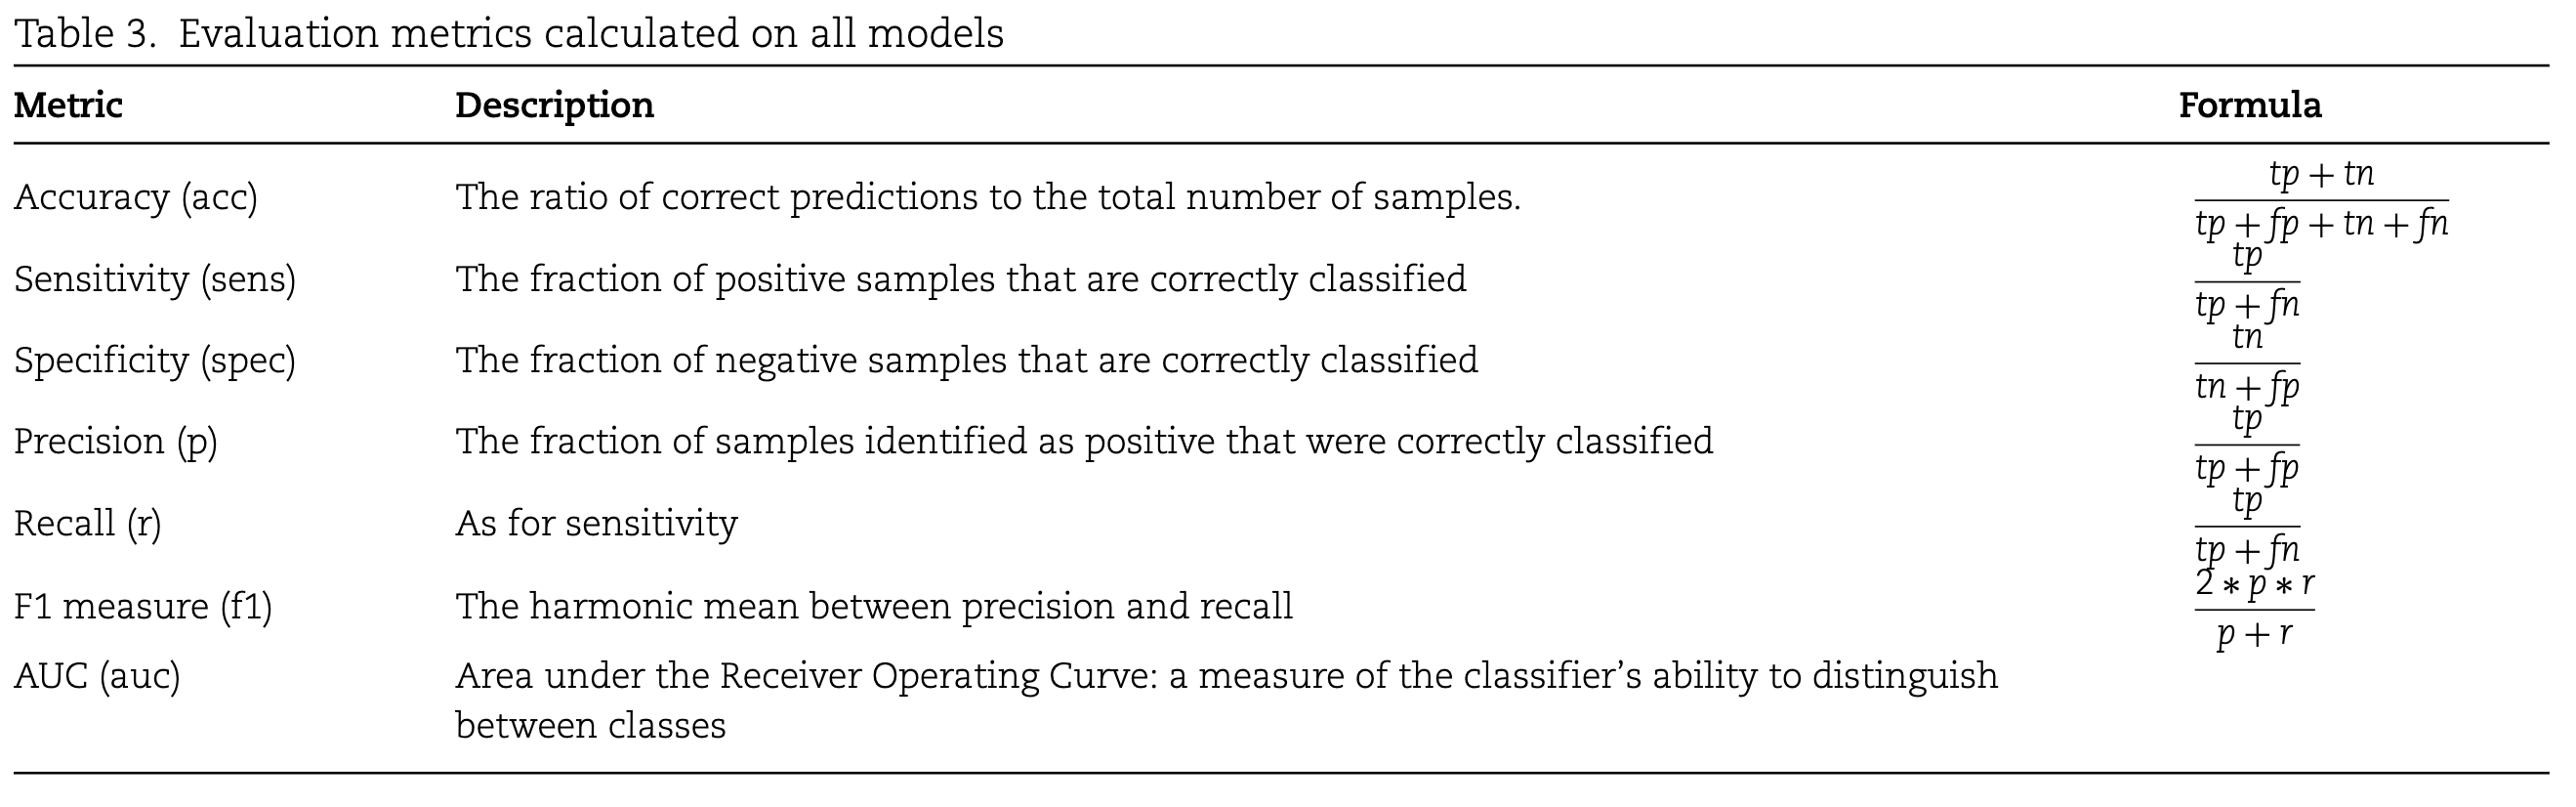
\includegraphics[width=1\textwidth]{assets/evaluation_metrics.png}
\end{figure}
\end{frame}

\begin{frame}{Individual vs. Multi-modal Performance}
\begin{figure}[H]
  \centering
  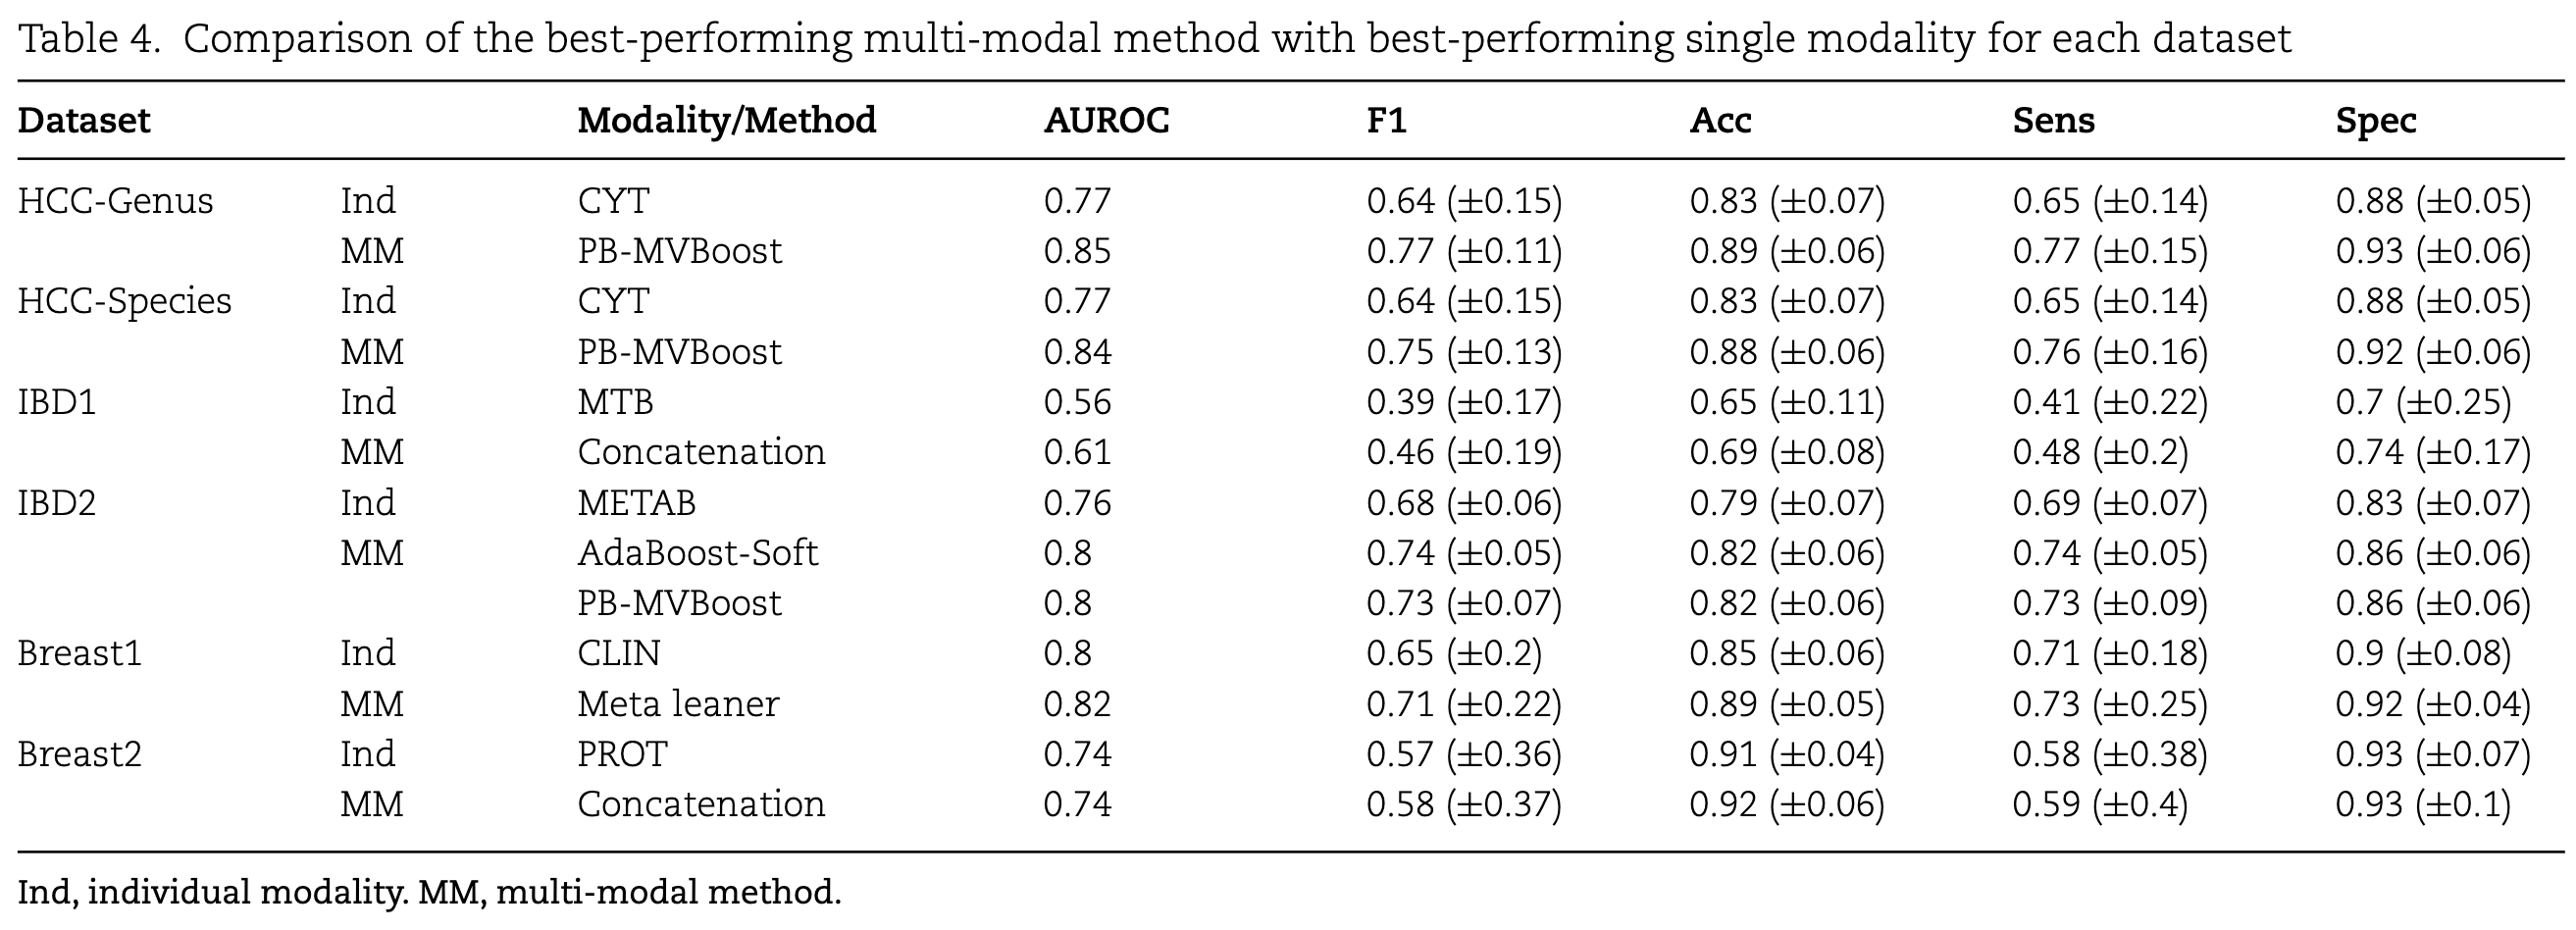
\includegraphics[width=1\textwidth]{assets/ind_mm.png}
\end{figure}

\alert{Multi-modal integration provides consistent improvements}
\end{frame}

\begin{frame}{Feature Selection Stability}
\begin{itemize}
\item \alert{Concatenation}: Least stable feature selection
\item \alert{PB-MVBoost}: Highest stability and accuracy
\item \alert{AdaBoost (soft vote)}: Good balance of stability and signature length
\item Integration methods overcome high-dimensional instability
\end{itemize}

\begin{block}{Clinical Signature Characteristics}
Desirable properties:
\begin{itemize}
\item Shorter signature length
\item Fewer modalities required
\item High stability and accuracy
\item Clinical interpretability
\end{itemize}
\end{block}
\end{frame}

\begin{frame}{Optimal Modality Subset}
  \begin{figure}[H]
    \centering
    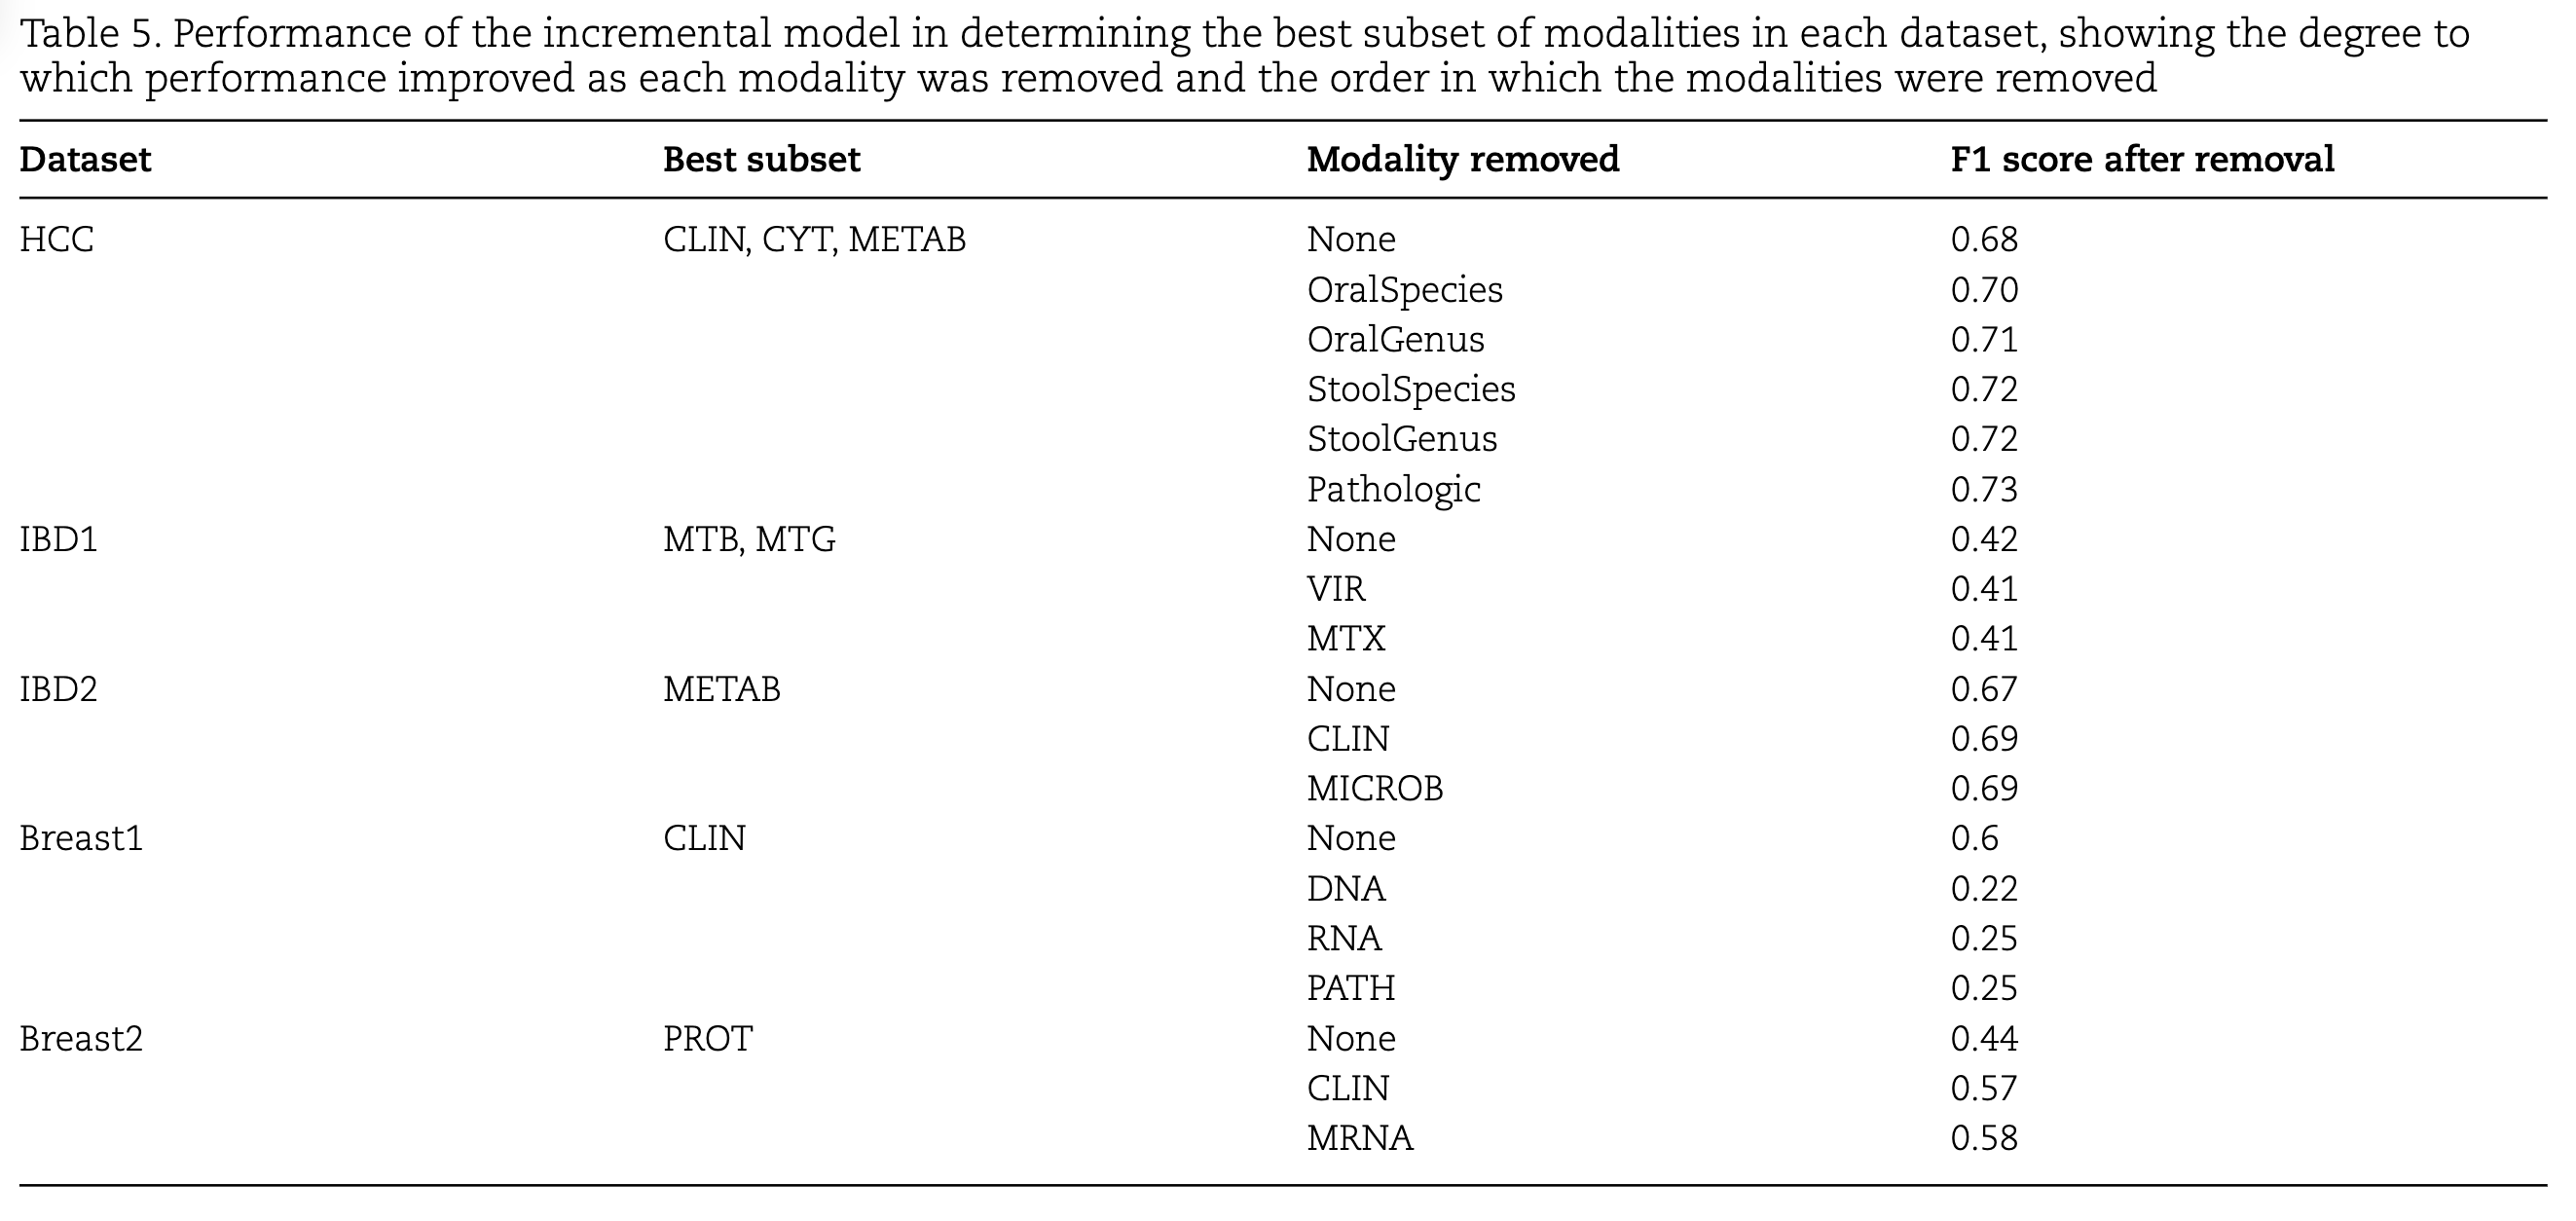
\includegraphics[width=1\textwidth]{assets/perform_sub.png}
  \end{figure}
\end{frame}

\begin{frame}{Optimal Modality Subset}
  \begin{figure}[H]
    \centering
    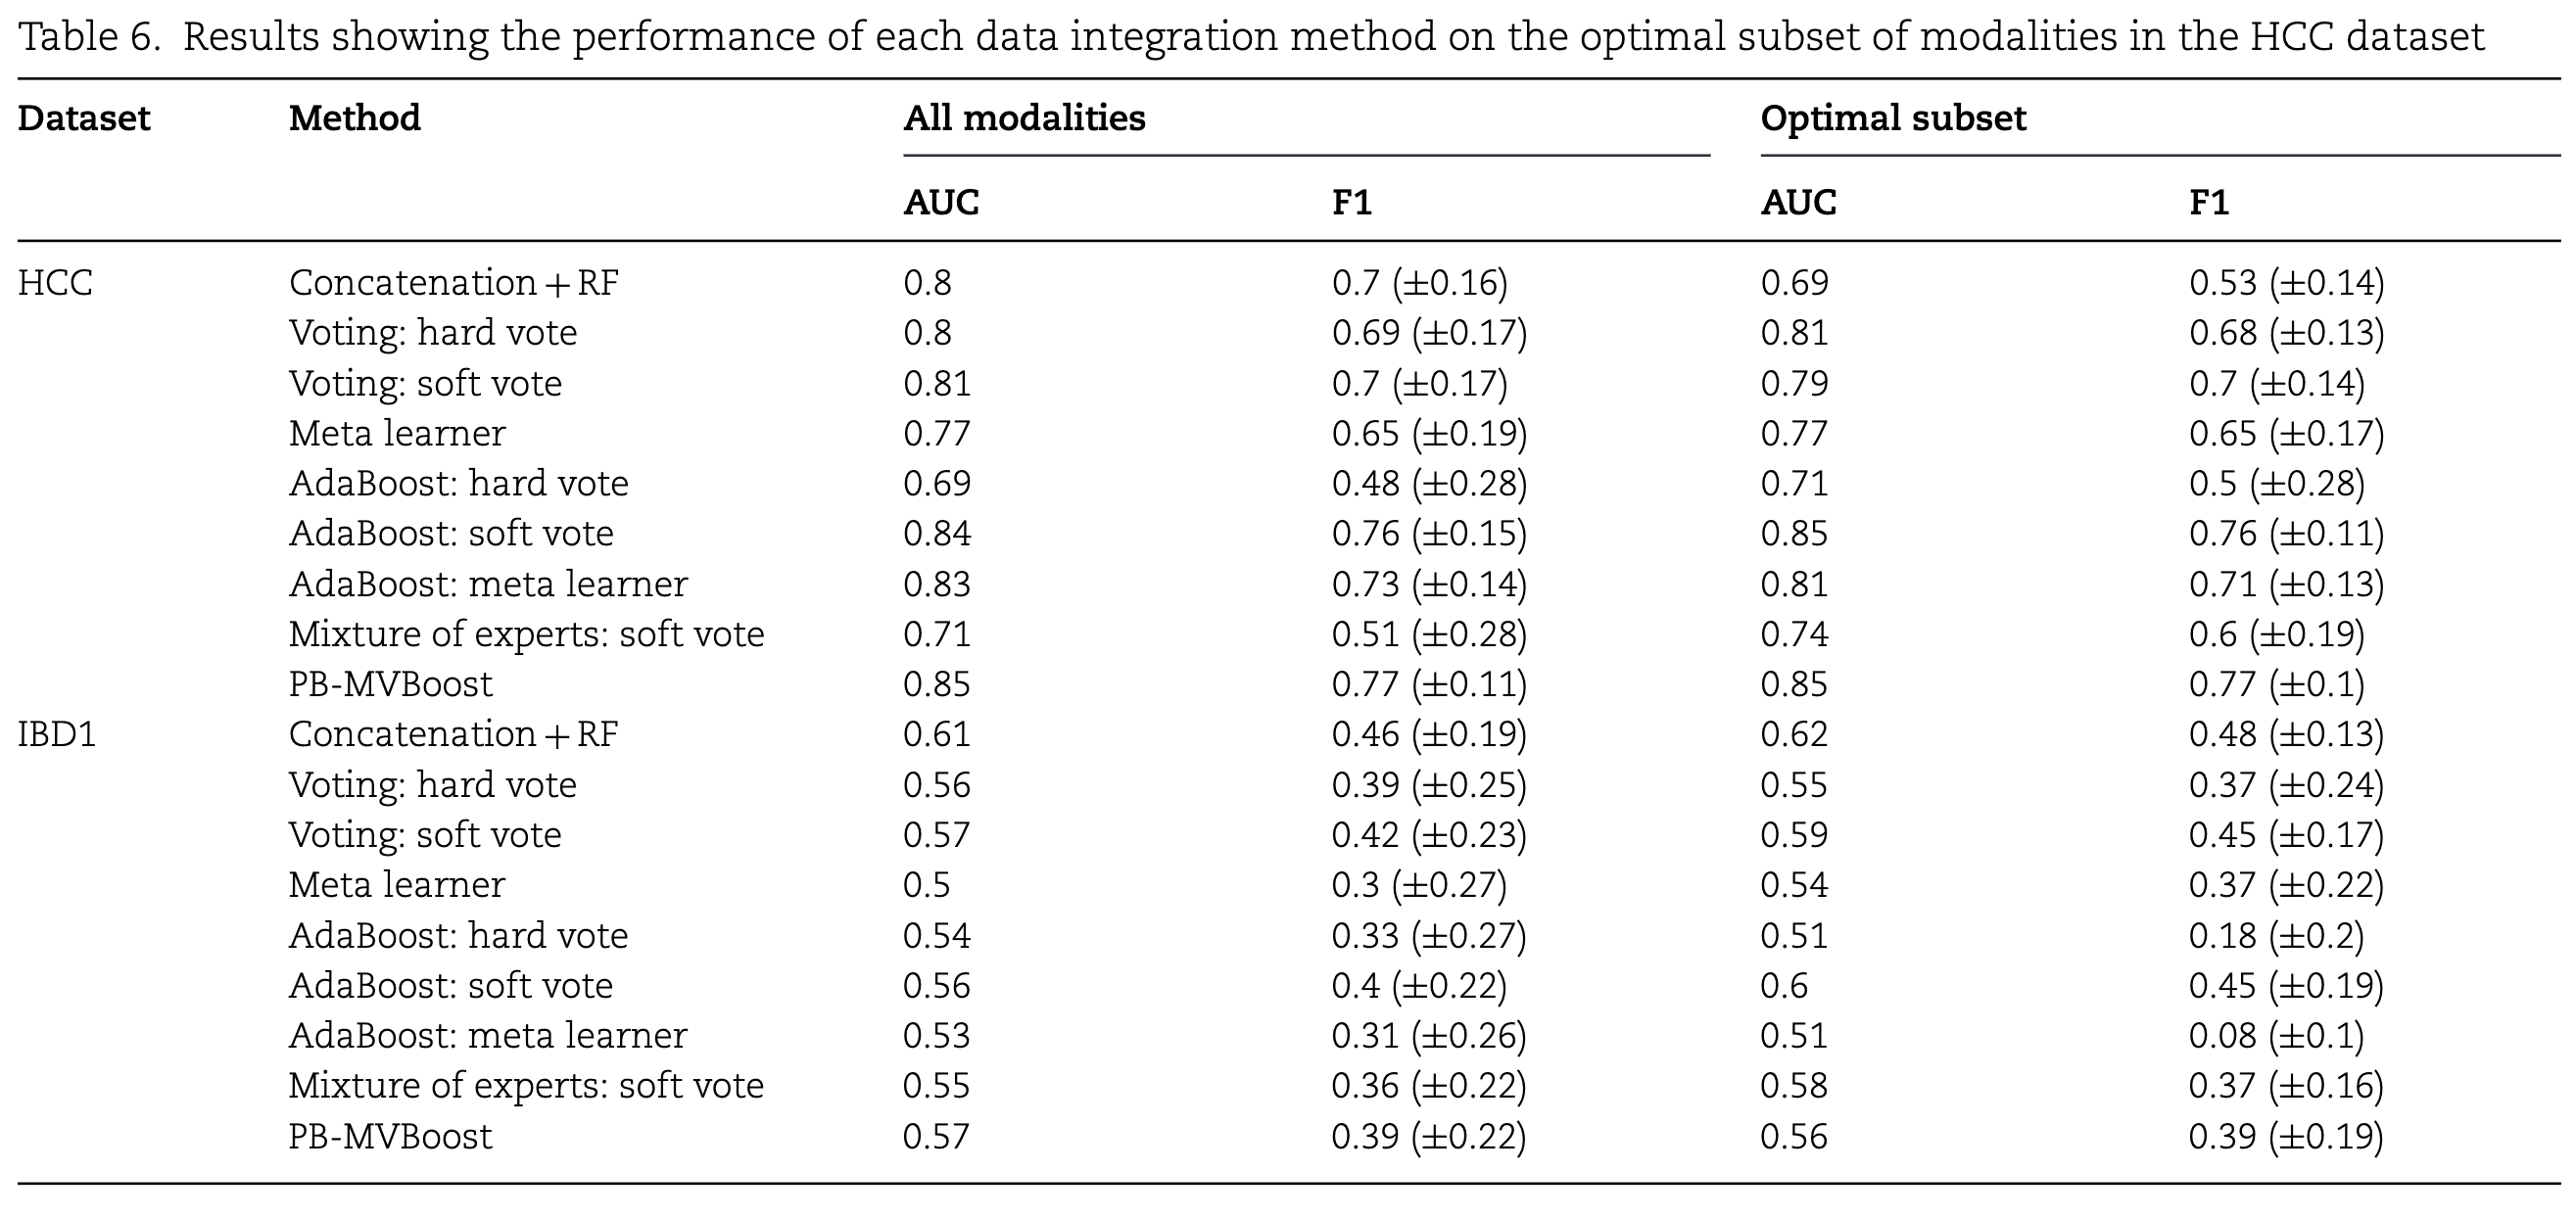
\includegraphics[width=1\textwidth]{assets/perform_data_inte.png}
  \end{figure}
\end{frame}

\begin{frame}{Optimal Modality Subset}
\begin{itemize}
\item \alert{Incremental model}: Determines optimal modality subset
\item Some datasets achieve \alert{equal performance} with fewer modalities
\item \alert{Clinical benefit}: Fewer tests required
\item Reduces cost and complexity
\end{itemize}

\begin{block}{Example: HCC Dataset}
\begin{itemize}
\item Full set: 7 modalities
\item Optimal subset: 4 modalities
\item Performance maintained with 43\% fewer tests
\end{itemize}
\end{block}
\end{frame}

\section{Discussion}

\begin{frame}{Key Findings}
\begin{itemize}[<+->]
\item \alert{Boosting methods superior}: PB-MVBoost and AdaBoost excel
\item \alert{Soft voting better}: More nuanced than hard voting
\item \alert{Multi-modal benefit}: Complementary information utilization
\item \alert{Stability matters}: Feature selection consistency crucial
\item \alert{Modality optimization}: Not all modalities equally valuable
\end{itemize}
\end{frame}

\begin{frame}{Why Boosting Works}
\begin{columns}
\begin{column}{0.6\textwidth}
\begin{itemize}
\item \alert{Reduces overfitting}
  \begin{itemize}
  \item Sequential weak learners
  \item Focus on difficult samples
  \end{itemize}
\item \alert{Modality weighting}
  \begin{itemize}
  \item Prioritizes predictive modalities
  \item Learned importance scores
  \end{itemize}
\item \alert{High-dimensional suitability}
  \begin{itemize}
  \item Designed for challenging datasets
  \item Small sample, large feature spaces
  \end{itemize}
\end{itemize}
\end{column}
\begin{column}{0.4\textwidth}
\begin{block}{Contrast}
Other methods give equal weight to all modalities, potentially diluting predictive power
\end{block}
\end{column}
\end{columns}
\end{frame}

\begin{frame}{Clinical Implications}
\begin{itemize}
\item \alert{Personalized medicine}: Better patient stratification
\item \alert{Biomarker discovery}: Stable feature signatures
\item \alert{Cost reduction}: Optimal modality subsets
\item \alert{Diagnostic efficiency}: Fewer required tests
\item \alert{Mechanistic insights}: Multi-modal feature importance
\end{itemize}

\begin{block}{Future Applications}
\begin{itemize}
\item Drug response prediction
\item Disease progression monitoring
\item Treatment selection guidance
\end{itemize}
\end{block}
\end{frame}

\section{Conclusion}

\begin{frame}{Best Practices for Multi-Modal Integration}
\begin{enumerate}
\item \alert{Examine individual modalities} first
  \begin{itemize}
  \item Identify most predictive modalities
  \end{itemize}
\item \alert{Apply incremental method}
  \begin{itemize}
  \item Determine optimal modality subset
  \end{itemize}
\item \alert{Use boosting methods}
  \begin{itemize}
  \item PB-MVBoost or AdaBoost with soft vote
  \end{itemize}
\item \alert{Consider stability}
  \begin{itemize}
  \item Balance accuracy and feature consistency
  \end{itemize}
\item \alert{Validate across datasets}
  \begin{itemize}
  \item Ensure generalizability
  \end{itemize}
\end{enumerate}
\end{frame}



% \begin{frame}{Summary}
% \begin{itemize}
% \item \alert{Comprehensive evaluation} of late integration methods
% \item \alert{PB-MVBoost and AdaBoost} emerge as top performers
% \item \alert{Multi-modal superior} to individual modalities
% \item \alert{Feature stability} crucial for clinical applications
% \item \alert{Modality optimization} reduces testing burden
% \end{itemize}

% \begin{block}{Main Contribution}
% First systematic comparison of ensemble methods for multi-modal, multi-class clinical data with focus on late integration strategies
% \end{block}
% \end{frame}

\begin{frame}{Future Work}
\begin{itemize}
\item \alert{Deep learning integration}
  \begin{itemize}
  \item Neural network ensemble methods
  \end{itemize}
\item \alert{Longitudinal data}
  \begin{itemize}
  \item Temporal multi-modal analysis
  \end{itemize}
\item \alert{Federated learning}
  \begin{itemize}
  \item Multi-center collaborative models
  \end{itemize}
\item \alert{Interpretability enhancement}
  \begin{itemize}
  \item Explainable AI for clinical decision support
  \end{itemize}
\item \alert{Real-world validation}
  \begin{itemize}
  \item Prospective clinical studies
  \end{itemize}
\end{itemize}
\end{frame}

% \footlinecolor{sintefgreen}
% \begin{frame}{Thank You}
% \begin{center}
% {\Large Questions \& Discussion}

% \vspace{1cm}

% \begin{itemize}
% \item Email: \hrefcol{mailto:yinchao@example.com}{yinchao@example.com}
% \item Code: Available upon request
% \item Datasets: Public datasets used with proper citations
% \end{itemize}
% \end{center}
% \end{frame}

\backmatter
\end{document}
